\documentclass[a4paper,11pt,dvipdfmx]{ujarticle}
% パッケージ
\usepackage{graphicx}
\usepackage{url}
% レイアウト指定を記述したファイルの読み込み
\input{layout}

% タイトルと氏名を変更せよ.
\title{日本におけるデジタル化の状況}
\author{G584882025 宮本 燿粋}

\begin{document}

\maketitle %ここにタイトルが入る

% ここから本文
\section{ブロードバンドの整備状況}
OECDによるブロードバンド回線の普及に関する調査\cite{oecd}によると、図\ref{fig:ランキング}に示すように、
日本における100人あたりの光ファイバー回線の加入者数は29.9で、韓国、スウェーデン、ノルウェーに続いて
第4位になっている。

% 図の挿入
% 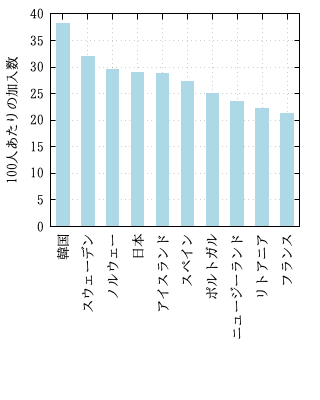
\includegraphics{fig11.png}
% を

\begin{figure}[htbp]
    \centering
    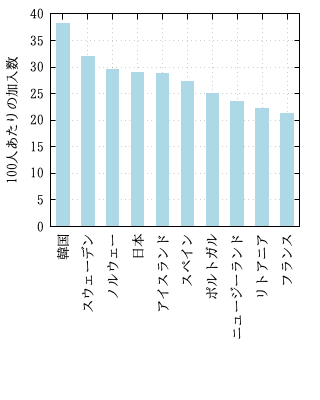
\includegraphics{fig11.png}
    \caption{光ファイバー回線の加入者数(百人あたり)}\label{fig:ランキング}
\end{figure}

% で囲み
% \caption{}
% で図のタイトルを入れる.
% \label{}
% を使って図番号が参照できるようにする
% また,
% \centering
% で図が中央に来るようにする

% ーーー
% 節見出し(2)
\section{デジタル競争力ランキング}

国際経営研究所(IMD)の調査\cite{imd}によると、日本のデジタル競争力のランキングは表\ref{tbl:デジタル}に示すように、
調査対象の64カ国中、総合で28位、準備分野で27位となっている。

% 本文(2)

\begin{table}[htbp]
        \centering
        \caption{デジタル競争力ランキング(64カ国中)}
        \label{tbl:デジタル}
        \begin{tabular}{|c|c|c|}
            \hline
            国 & 総合 & 準備 \\
            \hline
            米国 & 1位 & 1位 \\
            \hline
            香港 & 2位 & 10位 \\
            \hline
            スウェーデン & 3位 & 6位 \\
            \hline
            デンマーク & 4位 & 2位 \\
            \hline
            シンガポール & 5位 & 11位 \\
            \hline
            \hline
            韓国 & 12位 & 5位 \\
            \hline
            中国 & 15位 & 17位 \\
            \hline
            \hline
            日本 & 28位 & 27位 \\
            \hline
        \end{tabular}
\end{table}


% 表の挿入
% \begin{tabular}
% \end{tabular}    
% による表の記述を 
% \begin{table}[htbp]
% \end{table}
% で囲み
% \caption{}
% で表のタイトルを入れる.
% \label{}
% を使って表番号が参照できるようにする
% また,
% \centering
% で表が中央に来るようにする

% ーーー
% 見出し(3)
\section{考察}
\begin{itemize}
    \item 日本は核家族化が進んでいるが、それでも一つの家に親類と住むことは珍しくないので、家に一回線あれば十分な光回線の100人あたりの加入者が少なくなっているのではないか。
    \item 日本のデジタル競争力が低いのは、コンピュータで主に使われる英語を使える人が他の国と比べて少ないのと関係があるのではないか。
\end{itemize}

% 考察
%
% \begin{itemize}
% \end{itemize}
% を使って箇条書きで記述する

% ここに参考文献が入る
%
\bibliographystyle{junsrt}
\bibliography{exercise.bib}

\end{document}